% SPDX-FileCopyrightText: 2023 SAP SE
%
% SPDX-License-Identifier: Apache-2.0
%
% This file is part of FEDEM - https://openfedem.org

%%%%%%%%%%%%%%%%%%%%%%%%%%%%%%%%%%%%%%%%%%%%%%%%%%%%%%%%%%%%%%%%%%%%%%%%%%%%%%%%
%
% FEDEM Theory Guide.
%
%%%%%%%%%%%%%%%%%%%%%%%%%%%%%%%%%%%%%%%%%%%%%%%%%%%%%%%%%%%%%%%%%%%%%%%%%%%%%%%%

\def\Eqnref#1{Equation~\eqref{#1}}
\def\Fi{{\bf F}^{\rm I}}
\def\Fd{{\bf F}^{\rm D}}
\def\Fs{{\bf F}^{\rm S}}
\def\Q {{\bf Q}}
\def\kp1{{k+1}}
\def\ls#1{{}^{#1}}
\def\dr{\delta{\mf r}}
\def\ddr{\delta\dot{\mf r}}
\def\dddr{\delta\ddot{\mf r}}

\chapter{Dynamics Simulation}
\label{c:Dynamics Simulation}

%%%%%%%%%%%%%%%%%%%%%%%%%%%%%%%%%%%%%%%%%%%%%%%%%%%%%%%%%%%%%%%%%%%%%%%%%%%%%%%%
\section{Dynamics equation on incremental form}
\label{s:Dynamics equation on incremental form}

The equation of dynamic equilibrium at time $t$ may be written
%
\begin{equation}
{\mf R} \left( t, {\mf r}, \dot{\mf r}, \ddot{\mf r} \right) \;=\; {\mf 0}
\label{eq:31}
\end{equation}
%
or
%
\begin{equation}
\Fi \left( t, {\mf r}, \dot{\mf r}, \ddot{\mf r} \right) \,+\,
\Fd \left( t, {\mf r}, \dot{\mf r}, \ddot{\mf r} \right) \,+\,
\Fs \left( t, {\mf r}, \dot{\mf r}, \ddot{\mf r} \right) \,-\,
\Q  \left( t, {\mf r}, \dot{\mf r}, \ddot{\mf r} \right) \;=\; {\mf 0}
\label{eq:32}
\end{equation}
%
where
%
\begin{namelist}{XX}
\item[$\Fi$] represents inertia forces,
\iftoggle{publicedition}{}{% The following is for the in-house edition only.
with the optional inclusion of inertia force correction terms, as defined in
Section~\ref{subs:Correction to FE inertia forces}
} % End in-house edition only
\item[$\Fd$] represents damping forces
\item[$\Fs$] represents internal elastic forces
\item[$\Q$] represents input loads (forces and torques)
and gravitational forces
\end{namelist}
%
\Eqnref{eq:32} is integrated in time with a time increment length of $h$.
At time $t_k$, this equation of equilibrium may be written
%
\begin{equation}
\Fi_k + \Fd_k + \Fs_k \;=\; \Q_k
\label{eq:DynEquil}
\end{equation}

Since \eqnref{eq:DynEquil} has to be satisfied at all times, we can subtract
this equation from the same equation at time $t_\kp1=t_k+h$ to produce the
equation of motion on incremental form, as follows
%
\begin{equation}
\left[ \Fi_\kp1 - \Fi_k \right] \,+\,
\left[ \Fd_\kp1 - \Fd_k \right] \,+\,
\left[ \Fs_\kp1 - \Fs_k \right] \;=\; \Q_\kp1 - \Q_k
\end{equation}
%
or
%
\begin{equation}
\Delta\Fi_k + \Delta\Fd_k + \Delta\Fs_k \;=\; \Delta\Q_k
\label{eq:DynEquilIncForm}
\end{equation}
%
In the following,
the different terms of \eqnref{eq:DynEquilIncForm} are expanded.

The inertia, damping and stiffness relationships are estimated by a linear
approximation around the starting position for each time increment.
Incremental system matrices are then generated for that configuration.
Equilibrium iterations are next used to reduce the error in this approximation.
The exact incremental system matrices, called tangent matrices, are functions
of the unknown displacement increments and cannot be generated in advance.

The incremental inertia forces from \eqnref{eq:DynEquilIncForm} may be written
%
\begin{equation}
\Delta\Fi_k \;=\; \Fi_\kp1 - \Fi_k \;=\; {\mf M}_k \Delta\ddot{\mf r}_k
\label{eq:37}
\end{equation}
%
where ${\mf M}_k$ is the system mass matrix at the beginning of time
increment $k$, and $\Delta\ddot{\mf r}_k = \ddot{\mf r}_\kp1 - \ddot{\mf r}_k$
represents the change in acceleration during that time increment.
The system mass matrix may be constant or a function of the displacement
${\mf r}$, depending on the element mass representation used.
The element mass matrices are constant, but undergo a geometric transformation
before they are added into the system matrix.
If a lumped mass representation is chosen, the element mass matrix is diagonal
and the geometric transformations have no effect.
Then the system mass matrix will be diagonal and constant during integration.

The incremental damping forces from \eqnref{eq:DynEquilIncForm} may be written
%
\begin{equation}
\Delta\Fd_k \;=\; \Fd_\kp1 - \Fd_k \;=\; {\mf C}_k \Delta\dot{\mf r}_k
\label{eq:38}
\end{equation}
%
where ${\mf C}_k$ is the system damping matrix at the beginning of time
increment $k$, and $\Delta\dot{\mf r}_k = \dot{\mf r}_\kp1 - \dot{\mf r}_k$
represents the change in velocity during that time increment.
The system damping matrix may be constant or a function of the displacement
${\mf r}$.
If the damping matrix is diagonal, the damping matrix will not be affected by
the geometric transformation and remains constant.

The incremental elastic forces from \eqnref{eq:DynEquilIncForm} may be written
%
\begin{equation}
\Delta\Fs_k \;=\; \Fs_\kp1 - \Fs_k \;=\; {\mf K}_k \Delta{\mf r}_k
\label{eq:39}
\end{equation}
%
where ${\mf K}_k$ is the system stiffness matrix at the beginning of time
increment $k$, and $\Delta{\mf r} = {\mf r}_\kp1 - {\mf r}_k$ represents the
associated displacement increment.
The system stiffness matrix is in general a function of the displacement vector.

The incremental dynamic equation of motion~(\ref{eq:DynEquilIncForm}) can now be
written on the linearized form
%
\begin{equation}
{\mf M}_k \Delta\ddot{\mf r}_k +
{\mf C}_k  \Delta\dot{\mf r}_k +
{\mf K}_k      \Delta{\mf r}_k \;=\; \Delta\Q_k
\label{eq:310}
\end{equation}
%
The matrices ${\mf M}_k$, ${\mf C}_k$ and ${\mf K}_k$ may be recalculated for
each time increment and iteration of the solution process.
Solving \eqnref{eq:310} using a time integration algorithm, such as the Newmark
method, gives $\Delta{\mf r}_k,\Delta\dot{\mf r}_k$, and $\Delta\ddot{\mf r}_k$.
Therefore, the total solution at the end of the increment is
%
\begin{equation}
\eqalign{
     {\mf r}_\kp1 \;=\;\; &      {\mf r}_k +      \Delta{\mf r}_k \cr
 \dot{\mf r}_\kp1 \;=\;\; &  \dot{\mf r}_k +  \Delta\dot{\mf r}_k \cr
\ddot{\mf r}_\kp1 \;=\;\; & \ddot{\mf r}_k + \Delta\ddot{\mf r}_k }
\end{equation}

This solution may be used to calculate the forces $\Fi_\kp1$, $\Fd_\kp1$ and
$\Fs_\kp1$.
However, due to the linear approximation there will be unbalanced forces at the
end of the increment, given by
%
\begin{equation}
\hat{\mf R}_\kp1 \;=\; \Q_\kp1 - \left[ \Fi_\kp1 + \Fd_\kp1 + \Fs_\kp1 \right]
\end{equation}
%
These residual forces may be added to the load increment for the next step
%
\begin{equation}
\Delta\hat\Q_k \;=\; \Delta\Q_k + \hat{\mf R}_k \;=\;
\Q_\kp1 - \left[ \Fi_k + \Fd_k + \Fs_k \right]
\end{equation}
%
Replacing $\Delta\Q_k$ by $\Delta\hat\Q_k$, \eqnref{eq:310} may then be written
%
\begin{equation}
{\mf M}_k \Delta\ddot{\mf r}_k +
{\mf C}_k  \Delta\dot{\mf r}_k +
{\mf K}_k      \Delta{\mf r}_k \;=\;
\Q_\kp1 - \left[ \Fi_k + \Fd_k + \Fs_k \right]
\label{eq:314}
\end{equation}

%%%%%%%%%%%%%%%%%%%%%%%%%%%%%%%%%%%%%%%%%%%%%%%%%%%%%%%%%%%%%%%%%%%%%%%%%%%%%%%%
\section{Newmark time integration}
\label{s:Newmark time integration}

The Newmark $\beta$-family of algorithms is used for time integration in Fedem.
The basis for the Newmark method is the following update scheme
%
\begin{eqnarray}
{\mf r}_\kp1 &=& {\mf r}_k + h \dot{\mf r}_k + \left(\frac{1}{2}-\beta\right)
h^2 \ddot{\mf r}_k + \beta
h^2 \ddot{\mf r}_\kp1
\label{eq:NewmarkBasis} \\[1mm]
\dot{\mf r}_\kp1 &=& \dot{\mf r}_k +
(1-\gamma) h \ddot{\mf r}_k + \gamma h \ddot{\mf r}_\kp1
\end{eqnarray}
%
where $\beta$ and $\gamma$ are integration parameters (see
Section~\ref{subs:Stability and accuracy}) and $h$ is the time increment length.
These equations may be rewritten into the incremental forms
%
\begin{eqnarray}
{\mf r}_\kp1 \;=\; {\mf r}_k + \Delta{\mf r}_k & \text{where} &
\Delta{\mf r}_k \;=\; h\dot{\mf r}_k + \frac{h^2}{2} \ddot{\mf r}_k +
\beta h^2 \Delta\ddot{\mf r}_k
\label{eq:321} \\
\dot{\mf r}_\kp1 \;=\; \dot{\mf r}_k + \Delta\dot{\mf r}_k & \text{where} &
\Delta\dot{\mf r}_k \;=\; h\ddot{\mf r}_k + \gamma h\Delta\ddot{\mf r}_k
\label{eq:320}
\end{eqnarray}

The increment in velocity and acceleration can now be expressed as functions of
the displacement increment and known quantities at time $t_k$.
With $\Delta\ddot{\mf r}_k = \ddot{\mf r}_\kp1 - \ddot{\mf r}_k$,
\eqnref{eq:321} produces
%
\begin{equation}
\eqalign{
\ddot{\mf r}_\kp1 \;=\; \ddot{\mf r}_k + \Delta\ddot{\mf r}_k \;=\;\; &
\ddot{\mf r}_k +
\frac{1}{\beta h^2}\Delta{\mf r}_k -
\frac{1}{\beta h} \dot{\mf r}_k -
\frac{1}{2\beta} \ddot{\mf r}_k \cr =\;\; &
\frac{1}{\beta h^2} \Delta{\mf r}_k - {\mf a}_k
}\label{eq:322}
\end{equation}
%
where
%
\begin{equation}
{\mf a}_k \;=\; \frac{1}{\beta h}\dot{\mf r}_k +
\left( \frac{1}{2\beta} - 1 \right) \ddot{\mf r}_k
\label{eq:323}
\end{equation}
%
Combining \eqnref{eq:320} with \eqnref{eq:322} yields
%
\begin{equation}
\eqalign{
\dot{\mf r}_\kp1 \;=\; \dot{\mf r}_k + \Delta\dot{\mf r}_k \;=\;\; &
\dot{\mf r}_k +
\frac{\gamma}{\beta h} \Delta{\mf r}_k -
\frac{\gamma}{\beta} \dot{\mf r}_k -
\left( \frac{\gamma h}{2\beta} - h \right) \ddot{\mf r}_k \cr =\;\; &
\frac{\gamma}{\beta h} \Delta{\mf r}_k - {\mf d}_k
}\label{eq:324}
\end{equation}
%
where
%
\begin{equation}
{\mf d}_k \;=\; \left( \frac{\gamma}{\beta} -1 \right) \dot{\mf r}_k +
\left( \frac{\gamma}{2\beta} - 1 \right) h \ddot{\mf r}_k
\label{eq:325}
\end{equation}

By inserting \eqsref{eq:322}{eq:324} into \eqnref{eq:314}, we now get
%
\begin{equation}
{\mf N}_k \Delta{\mf r}_k \;=\; \hat{\mf R}_k
\label{eq:326}
\end{equation}
%
where the Newton matrix is
%
\begin{equation}
{\mf N}_k \;=\; {\mf K}_k +
\frac{\gamma}{\beta h}{\mf C}_k +
\frac{1}{\beta h^2}{\mf M}_k
\label{eq:327}
\end{equation}
%
and the right-hand-side vector is
%
\begin{equation}
\hat{\mf R}_k \;=\; \Q_\kp1 - \left[
\Fi_k + \Fd_k + \Fs_k \right] +
{\mf M}_k \left[ {\mf a}_k + \ddot{\mf r}_k \right] +
{\mf C}_k \left[ {\mf d}_k + \dot{\mf r}_k \right]
\label{eq:328}
\end{equation}
%
The evaluation of the system Newton matrix, ${\mf N}_k$, is covered by
Section~\ref{s:Evaluation of the Newton matrix}, whereas the external loading,
$\Q_\kp1$, and the internal inertia, damping, and elastic forces, $\Fi_k$,
$\Fd_k$ and $\Fs_k$, are covered by
Section~\ref{s:Evaluation of the force vector}.

\subsection{Stability and accuracy}
\label{subs:Stability and accuracy}

The integration parameters $\gamma$ and $\beta$ are selected for controlling
the stability, accuracy and efficiency of the integration process.
For the linear case, the method is unconditionally stable for
%
\begin{equation}
\gamma \geq \frac{1}{2}
\qquad\text{and}\qquad
\beta \geq \frac{1}{4} \left( \gamma + \frac{1}{2} \right)^2
\label{eq:335}
\end{equation}
%
For smaller $\beta$-values, the method is only conditionally stable.
The stability criterion is
%
\begin{equation}
h_{\rm cr} \;=\; \frac{T}{2\pi} \left( \frac{1}{4}
\left( \gamma + \frac{1}{2} \right)^2 - \beta \right)^{-\frac{1}{2}}
\label{eq:336}
\end{equation}
%
where $h_{\rm cr}$ is the critical time increment size and $T$ is the period for
the highest frequency in the model.

The parameter $\gamma$ may be selected to introduce artificial damping into the
integration process.
$\gamma > \frac{1}{2}$ gives positive artificial damping; in other words,
the amplitude will decay with increasing $k$.
$\gamma < \frac{1}{2}$ gives negative artificial damping, i.e.,
the amplitude will increase with increasing $k$.
$\gamma = \frac{1}{2}$ gives no artificial damping.
Unfortunately, numerical (algorithmic) damping can not be introduced without
loss off accuracy, and using a value of $\gamma\neq\frac{1}{2}$ will make the
algorithm only first order accurate.
Consequently, $\gamma=\frac{1}{2}$ is often the selection.
In this case, the Newmark $\beta$-family includes the following methods
%
\begin{namelist}{XXXX}
\item[$\beta=0$] The second central difference method with $h_{\rm cr} = 0.318T$
\item[$\beta=\frac{1}{12}$] Fox-Goodwins method with $h_{\rm cr} = 0.389T$
\item[$\beta=\frac{1}{6}$] Linear acceleration with $h_{\rm cr} = 0.551T$
\item[$\beta=\frac{1}{4}$] Constant average acceleration (trapezoid method),
which is unconditionally stable for linear systems
\end{namelist}

Fedem is using $\gamma=\frac{1}{2}$ and $\beta=\frac{1}{4}$ for its Newmark
integration algorithm.
This constitutes a second order accurate integration with no numerical damping
for any frequencies.
Because of the lack of numerical damping, we must include structural damping to
the model to obtain stable integration with the Newmark algorithm.
We will usually include (mainly) stiffness proportional damping in order to
introduce dissipation of high-frequency modes, see
Section~\ref{s:Structural damping}.

%%%%%%%%%%%%%%%%%%%%%%%%%%%%%%%%%%%%%%%%%%%%%%%%%%%%%%%%%%%%%%%%%%%%%%%%%%%%%%%%
\section{Newton--Raphson iteration}
\label{s:Newton-Raphson iteration}

\Eqnref{eq:314} is an approximation of the equilibrium equation at time $t_\kp1$.
To achieve equilibrium at the end of the increment, so-called Newton--Raphson
iterations are used to minimize the error from the solution of this equation.

An iteration is formally conducted by replacing the right hand side of
\eqnref{eq:314} by the residual from the previous iteration,
$\ls{i-1}\hat{\mf R}_\kp1$,
and then solving for the correction $\dr_k$ to $\Delta{\mf r}_k$ from
%
\begin{equation}
\eqalign{
\ls{i}{\mf M}_k \ls{i}\dddr_k \,+\,
\ls{i}{\mf C}_k \ls{i}\ddr_k \,+\,
\ls{i}{\mf K}_k \ls{i}\dr_k \;=\;\; &
\ls{i-1}\Q_\kp1 \cr -\;\; & \left[
\ls{i-1}\Fi_\kp1 + \ls{i-1}\Fd_\kp1 + \ls{i-1}\Fs_\kp1
\right]
}\label{eq:NewtonDynEq}
\end{equation}
%
The superindex to the left of the symbols indicates the iteration number.
The displacement, velocity and acceleration increments are then corrected from
%
\begin{equation}
\eqalign{
  \ls{i}\Delta{\mf r}_k      \;=\;\; &
\ls{i-1}\Delta{\mf r}_k      \,+\, \ls{i}\dr_k \cr
  \ls{i}\Delta\dot{\mf r}_k  \;=\;\; &
\ls{i-1}\Delta\dot{\mf r}_k  \,+\, \ls{i}\ddr_k \cr
  \ls{i}\Delta\ddot{\mf r}_k \;=\;\; &
\ls{i-1}\Delta\ddot{\mf r}_k \,+\, \ls{i}\dddr_k
}\label{eq:316}
\end{equation}
%
The total displacement, velocity and acceleration vectors are updated through
%
\begin{equation}
\eqalign{
\ls{i}{\mf r}_\kp1      =\; & \ls{i-1}{\mf r}_\kp1      \,+\, \ls{i}\dr_k \cr
\ls{i}\dot{\mf r}_\kp1  =\; & \ls{i-1}\dot{\mf r}_\kp1  \,+\, \ls{i}\ddr_k \cr
\ls{i}\ddot{\mf r}_\kp1 =\; & \ls{i-1}\ddot{\mf r}_\kp1 \,+\, \ls{i}\dddr_k
}\label{eq:317}
\end{equation}

The improved displacement increment, given by \eqnref{eq:316}$_1$, is next
inserted into \eqsref{eq:322}{eq:324}, respectively, yielding
%
\begin{eqnarray}
\ls{i}\ddot{\mf r}_\kp1 &=&
\frac{1}{\beta h^2}\ls{i}\Delta{\mf r}_k - {\mf a}_k =
\frac{1}{\beta h^2}\left[\ls{i-1}\Delta{\mf r}_k + \ls{i}\dr_k\right] -
{\mf a}_k \\
\ls{i}\dot{\mf r}_\kp1 &=&
\frac{\gamma}{\beta h}\ls{i}\Delta{\mf r}_k - {\mf d}_k \hskip5pt =
\frac{\gamma}{\beta h}\left[\ls{i-1}\Delta{\mf r}_k + \ls{i}\dr_k\right]
 - {\mf d}_k
\end{eqnarray}
%
From this it follows that the iterative acceleration and velocity corrections
are given by, respectively
%
\begin{equation}
\ls{i}\dddr_k = \frac{1}{\beta h^2} \ls{i}\dr_k
\qquad\text{and}\qquad
\ls{i}\ddr_k = \frac{\gamma}{\beta h} \ls{i}\dr_k
\label{eq:NewmarkVelAndAccCorr}
\end{equation}

Combining \eqnref{eq:NewmarkVelAndAccCorr} with \eqnref{eq:NewtonDynEq} yields
%
\begin{equation}
\ls{i}{\mf N}_k \ls{i}\dr_k \;=\; \ls{i-1}\hat{\mf R}_k
\label{eq:NewmarkDispCorr}
\end{equation}
%
with
%
\begin{equation}
\ls{i}{\mf N}_k \;=\; \ls{i}{\mf K}_k +
\frac{\gamma}{\beta h} \ls{i}{\mf C}_k +
\frac{1}{\beta h^2} \ls{i}{\mf M}_k
\label{eq:333}
\end{equation}
%
and
%
\begin{equation}
\ls{i-1} \hat{\mf R}_k \;=\; \ls{i-1}\Q_\kp1 - \left[
\ls{i-1}\Fi_\kp1 + \ls{i-1}\Fd_\kp1 + \ls{i-1}\Fs_\kp1
\right]
\label{eq:residual}
\end{equation}

After updating the solution state through the \eqsref{eq:316}{eq:317},
the internal forces $\ls{i}\Fi_\kp1$, $\ls{i}\Fd_\kp1$ and $\ls{i}\Fs_\kp1$
can be calculated from the \meqsref{eq:37}{eq:39} and substituted into
\eqnref{eq:NewtonDynEq} to solve for the correction $\ls{i+1}\dr_k$
of the next iteration, and so on.

If the matrices ${\mf M}_k$, ${\mf C}_k$ and ${\mf K}_k$ are updated in each
iteration, this iteration process is called Newton--Raphson iteration.
If they all are left constant during the iterations, or only updated after some
iterations, the process is called modified Newton--Raphson iteration.
The coefficient matrix of the equation system~\eqref{eq:NewmarkDispCorr} is then
unchanged for those iterations and new triangularizations are avoided.
The iterations are repeated until the chosen convergence test is satisfied
(refer to Section~\ref{subs:Convergence criteria}).

% SPDX-FileCopyrightText: 2023 SAP SE
%
% SPDX-License-Identifier: Apache-2.0
%
% This file is part of FEDEM - https://openfedem.org

%%%%%%%%%%%%%%%%%%%%%%%%%%%%%%%%%%%%%%%%%%%%%%%%%%%%%%%%%%%%%%%%%%%%%%%%%%%%%%%%
%
% FEDEM Theory Guide.
%
%%%%%%%%%%%%%%%%%%%%%%%%%%%%%%%%%%%%%%%%%%%%%%%%%%%%%%%%%%%%%%%%%%%%%%%%%%%%%%%%

\subsection{Convergence criteria}
\label{subs:Convergence criteria}

Some criteria for terminating the equilibrium iterations governed by
\meqsref{eq:NewtonDynEq}{eq:317}, must be established.
They are typically based on some {\it norms} of the vector quantities involved.
When computing the norms, we have the problem of dealing with different units.
There are rotational and translational DOFs (typically measured in radians and
meters), as well as generalized DOFs associated with the component modes.

Changing the modeling units of length and translation from [m] to [mm] changes
the size of the translations with 3 orders of magnitude, whereas the rotations
remain the same.
Such a change of units should not affect the relative contribution of rotation
and translations to the norm of a displacement vector.

\subsubsection{Scaled vector norms}

In order to make the vector norms unit independent, we choose to use rotations
as the ``base'' displacement quantity since they are always measured in radians.
With a rigid rotation of unit magnitude as guiding displacement, an appropriate
scaling of the translations is then assumed to be $\frac{1}{L_\text{model}}$,
where $L_\text{model}$ is the largest dimension of the model itself.

Based on this, we define the scaled vector norm as
%
\begin{equation}
% Corrected by KMO 19.08.04 (see TT #2074)
\left\| {\mf v} \right\|_\text{scaled} \;=\;
\sqrt{\frac{\sum_i(w_i v_i)^2}{\sum_i w_i^2}}
\end{equation}
%
\begin{equation*}
\text{where}\quad\left\{\begin{array}{ll}
w_i = 1 & \text{if $i$ is rotational DOF} \\
w_i = \frac{1}{L_\text{model}} & \text{if $i$ is translational DOF} \\
w_i = 1 & \text{if $i$ is generalized DOF}
\end{array}\right.
\end{equation*}
%
Convergence criterias are now defined as
%
\begin{equation}
\left\| {\mf v} \right\|_\text{scaled} \leq \varepsilon_\textit{tol}
\end{equation}
%
where the vector ${\mf v}$ can be one of the following
%
\clearpage
\begin{namelist}{XXX}
%
\item[$\ls{i}\dr_k$] displacement correction
defined by \eqsref{eq:NewtonDynEq}{eq:NewmarkDispCorr}
%
\item[$\ls{i}\ddr_k$] velocity correction
defined by \eqsref{eq:NewtonDynEq}{eq:NewmarkVelAndAccCorr}\footnote{
For the scaled vector norm of the velocity correction we also have the option of
``relaxing'' the convergence criterion when the overall velocity of the
mechanism is large, i.e.,
\begin{equation*}
\varepsilon_{tol} \;=\; \varepsilon_{abs} +
\varepsilon_{vel}\left\|\dot{\mf v}\right\|
\end{equation*}}
%
\item[$\ls{i}\dddr_k$] acceleration correction
defined by \eqsref{eq:NewtonDynEq}{eq:NewmarkVelAndAccCorr}
%
\item[$\ls{i}\hat{\mf R}_k$] residual vector (unbalanced forces)
defined by \eqsref{eq:NewtonDynEq}{eq:residual}
%
\end{namelist}
%
The scaling factors are inverted for the force residual vector.

\remark{Velocity and acceleration corrections are computed from the displacement
correction as time step dependent scalings proportional to
$\frac{1}{h}$ and $\frac{1}{h^2}$ respectively,
as given by \eqnref{eq:NewmarkVelAndAccCorr}.
For small time steps, any noise in the displacement corrections gets greatly
magnified in the velocity and acceleration terms, and can lead to convergence
problems if the convergence criterion involves testing on the
velocity and acceleration corrections.}

\subsubsection{DOF type selective infinite norms}

The infinite norm of a vector is defined as
%
\begin{equation}
\left\|{\mf v}\right\|_{\infty} \;=\; \lim_{n\to\infty} \sqrt[n]{\sum_i |v_i^n|}
 \;=\; \max_{\forall i} |v_i|
\end{equation}
%
Because of the different DOF types (rotation, translation and component modes),
we define three different infinite norms of a mixed vector ${\mf v}$ as
%
\begin{equation}
\begin{array}{lcll}
\left\| {\mf v} \right\|_{\infty,\text{tran}} &=& \max|v_i| &
:\;\forall\; i \text{~being a translational DOF} \\
\left\| {\mf v} \right\|_{\infty,\text{rot}} &=& \max|v_i| &
:\;\forall\; i \text{~being a rotational DOF} \\
\left\| {\mf v} \right\|_{\infty,\text{gen}} &=& \max|v_i| &
:\;\forall\; i \text{~being a component mode DOF}
\end{array}
\end{equation}
%
Convergence criterias based on these norms are now defined as
%
\begin{equation}
\left\|{\mf v}\right\|_{\infty,\text{tran}} \leq \varepsilon_\textit{tol},\quad
\left\|{\mf v}\right\|_{\infty,\text{rot}} \leq \varepsilon_\textit{tol},\quad
\left\|{\mf v}\right\|_{\infty,\text{gen}} \leq \varepsilon_\textit{tol}
\end{equation}
%
where ${\mf v}$ can be the correction to the displacements $\ls{i}\dr_k$,
velocity $\ls{i}\ddr_k$, acceleration $\ls{i}\dddr_k$,
as well as the residual vector $\ls{i}\hat{\mf R}_k$.

\subsubsection{Energy norms}

The product of residual vector $\ls{i}\hat{\mf R}_k$ and displacement
correction $\ls{i}\dr_k$ form an incremental energy term.
The advantage of using this quantity in convergence testing is the automatic
same unit of energy for all DOFs regardless of translation/force,
rotation/torque, or generalized DOF/generalize force.

We define energy norm analogous to the infinite and scaled vector norms
respectively, as the max DOF energy and average energy
%
\begin{eqnarray}
\text{Max DOF energy:} &
E_{\max} =& \max_{j=1,n}
\left| \ls{i}\delta r_{kj} \ls{i}\hat{R}_{kj} \right| \\
\text{Average energy:} &
E_\text{avg} \;=& \frac{1}{n} \sum_{j=1,n}
\left| \ls{i}\delta r_{kj} \ls{i}\hat{R}_{kj} \right|
\end{eqnarray}
%
\remark{Structures close to a buckling state will often be close to force
equilibrium (low residual norm), while the displacements are largely
undetermined (high displacement correction norm).
Similarly, structures with very stiff members often are close to the correct
position (low displacement correction norm), whereas the unbalanced forces are
high (high residual norm).
Both of these cases can lead to convergence problems when the convergence
criterion is based on displacements and/or force equilibrium.
In these cases the energy norms often give a more ``balanced'' picture and can
improve stability in passing problem areas in the dynamics simulation.}


%%%%%%%%%%%%%%%%%%%%%%%%%%%%%%%%%%%%%%%%%%%%%%%%%%%%%%%%%%%%%%%%%%%%%%%%%%%%%%%%
\section{Newmark integration with numerical damping}
\label{s:Newmark integration with numerical damping}

\subsection{The Hilber--Hughes--Taylor method}
\label{subs:The Hilber--Hughes--Taylor method}

The $\alpha$-method by Hilber, Hughes and Taylor~\cite{HHT} circumvents the
problem of not being able to introduce numerical damping without a loss of
accuracy as in the traditional Newmark algorithm.
This is achieved by modifying the equilibrium \eqnref{eq:DynEquil}, as follows
%
\begin{equation}
\Fi_\kp1 +
(1+\alpha)\Fd_\kp1 - \alpha\Fd_k +
(1+\alpha)\Fs_\kp1 - \alpha\Fs_k \;=\;
(1+\alpha)\Q_\kp1  - \alpha\Q_k
\label{eq:NewmarkAlphaEquil}
\end{equation}
%
where $\alpha$ adjusts the amount of numerical damping.

The HHT-$\alpha$ method gives efficient high-frequency dissipation and is
unconditionally stable for parameters in the range
%
\begin{equation}
\alpha \in [-\frac{1}{3},0], \qquad
\gamma = \frac{1}{2}(1-2\alpha), \qquad\text{and}\qquad
\beta = \frac{1}{4}(1-\alpha)^2
\end{equation}
%
Fedem is using $\alpha = -0.1$, which gives $\gamma = 0.6$ and $\beta = 0.3025$.

\remark{For simulations involving high-speed rotations, the $\alpha$-method can
give less accurate estimates for the rigid body rotational velocities than the
standard Newmark method.
The latter method might give better results and allow larger time increments in
such cases.
Note, however, that the standard Newmark method requires more structural damping
than the $\alpha$-method.
With the use of stiffness proportional damping, no artificial damping against
the rigid body rotation is introduced.}

\Eqnref{eq:NewmarkAlphaEquil} can also be expressed as
%
\begin{equation}
\Fi_\kp1 \,+\, (1+\alpha)\Fd_\kp1 \,+\, (1+\alpha)\Fs_\kp1 \;=\;
(1+\alpha)\Q_\kp1 \,-\, \alpha\Fi_\text{actual}
\label{eq:HHTequil}
\end{equation}
%
where $\Fi_\text{actual}$ represents the actual inertia force at increment $k$,
computed from the equilibrium \eqnref{eq:DynEquil}, i.e.
%
\begin{equation}
\Fi_\text{actual} \;=\; \Q_k - \Fd_k - \Fs_k
\end{equation}
%
This modified equilibrium equation is integrated by the standard Newmark method.
Hence, the finite difference expressions~\eqref{eq:NewmarkBasis}--\eqref{eq:325}
are retained.

By inserting the internal force linearizations from \meqsref{eq:37}{eq:39} into
\eqnref{eq:HHTequil}, we obtain
%
\begin{equation}
\eqalign{
\Fi_k \,+\, {\mf M}_k\Delta\ddot{\mf r}_k \;\;+\;\; &
(1+\alpha)\left( \Fd_k + {\mf C}_k\Delta\dot{\mf r}_k \right) \cr +\;\; &
(1+\alpha)\left( \Fs_k + {\mf K}_k\Delta{\mf r}_k \right) \cr =\;\; &
(1+\alpha)\,\Q_\kp1 \,-\, \alpha\Fi_\text{actual} }
\end{equation}
%
or
%
\begin{equation}
\eqalign{
{\mf M}_k\Delta\ddot{\mf r}_k \;+\; &
(1+\alpha)\,{\mf C}_k\Delta\dot{\mf r}_k +
(1+\alpha)\,{\mf K}_k\Delta{\mf r}_k \cr =\; &
(1+\alpha)\left(\Q_\kp1 - \Fd_k - \Fs_k \right) - \Fi_k
-\alpha\Fi_\text{actual}
}\label{eq:IncHHTequil}
\end{equation}
%
Inserting the Newmark incremental acceleration and velocity expressions from
\eqsref{eq:322}{eq:324}, resepctively, into \eqnref{eq:IncHHTequil} now yields
%
\begin{equation}
\eqalign{
          {\mf M}_k&\left(
\frac{1}{\beta h^2} \Delta{\mf r}_k - {\mf a}_k - \ddot{\mf r}_k \right) \;+ \cr
(1+\alpha){\mf C}_k&\left(
\frac{\gamma}{\beta h} \Delta{\mf r}_k - {\mf d}_k - \dot{\mf r}_k \right) \;+ \cr
(1+\alpha){\mf K}_k&\Delta{\mf r}_k \;=\;
(1+\alpha)\left(\Q_\kp1 - \Fd_k - \Fs_k \right) - \Fi_k
-\alpha\Fi_\text{actual} }
\end{equation}
%
which after rearranging the known quantities on the right hand side becomes
%
\begin{equation}
{\mf N}_k \Delta{\mf r}_k \;=\; \widehat{\mf R}_k
\end{equation}
%
with
%
\begin{equation}
{\mf N}_k \;=\;
\frac{1}{\beta h^2}{\mf M}_k \;+\;
\frac{(1+\alpha)\gamma}{\beta h} {\mf C}_k \;+\;
(1+\alpha){\mf K}_k
\label{eq:NewtonHHT}
\end{equation}
%
and
%
\begin{equation}
\eqalign{
\widehat{\mf R}_k \;=\; & (1+\alpha)\left(
\Q_\kp1 + {\mf C}_k({\mf d}_k + \dot{\mf r}_k) - \Fd_k - \Fs_k \right) \cr +\; &
{\mf M}_k({\mf a}_k + \ddot{\mf r}_k) - \Fi_k - \alpha\Fi_\text{actual}
}\label{eq:PredictorHHT}
\end{equation}

If we assume that the inertia- and damping forces are linear with respect to the
total acceleration and velocity, respectively, we have that
$\Fd_k={\mf C}_k\dot{\mf r}_k$ and $\Fi_k={\mf M}_k\ddot{\mf r}_k$, and
\eqnref{eq:PredictorHHT} reduces to the following
%
\begin{equation}
\eqalign{
\widehat{\mf R}_k \;=\; & (1+\alpha)\left(
\Q_\kp1 + {\mf C}_k{\mf d}_k - \Fs_k \right) \;+\;
{\mf M}_k{\mf a}_k - \alpha\Fi_\text{actual}
}\label{eq:PredictorHHTsimplified}
\end{equation}
%
The \eqnref{eq:PredictorHHTsimplified} is used as the default force predictor
in Fedem, optionally also replacing $\Fi_\text{actual}$ by $\Fi_k$.
The linear assumption on the inertia- and damping- forces is a simplification
that should not matter much if the mass- and damping characteritiscs are
relatively constant during the simulation time.
However, for systems consisting of large bodies moving relative to each other,
like in contact problems, or systems with significant nonlinear damping,
like hydrodynamic drag, etc., it is worth considering using the full expression,
\eqnref{eq:PredictorHHT}.

\remark{A small error in the predictor force usually has no significance in
a nonlinear simulation with Newton--Raphson iterations, since then it will
iterate towards the correct solution in any case.
But if the predictor force is too far off, there is a risk of divergence,
or in the worst case, convergence towards an incorrect solution.}

For a linear system, the state at time $t_\kp1$ given by $\Delta{\mf r}_k$,
$\Delta\dot{\mf r}_k$ and $\Delta\ddot{\mf r}_k$, and the associated inertia,
damping and elastic forces forces $\Fi_\kp1$, $\Fd_\kp1$ and $\Fs_\kp1$,
respectively, will satisfy the equilibrium \eqnref{eq:HHTequil}.
However, for nonlinear systems the increments $\Delta{\mf r}_k$,
$\Delta\dot{\mf r}_k$ and $\Delta\ddot{\mf r}_k$ will in general not satisfy
\eqnref{eq:HHTequil}.
In order to ensure dynamic equilibrium before advancing to the next increment,
the dynamic residual seeks to be minimized through a similar Newton--Raphson
procedure as described in Section~\ref{s:Newton-Raphson iteration}.
Thus, in each iteration we have to solve the linearized system of equations
%
\begin{equation}
\ls{i}{\mf N}_k \ls{i}\Delta_k \;=\; \ls{i-1}\widehat{\mf R}_k
\end{equation}
%
where the Newton matrix $\ls{i}{\mf N}_k$ is the same as in
\eqnref{eq:NewtonHHT}, and the right-hand-side vector
$\ls{i-1}\widehat{\mf R}_k$ equals the residual from the previous iteration
%
\begin{equation}\small
\ls{i-1}\widehat{\mf R}_k \;=\; (1+\alpha)\left(
\ls{i-1}\Q_\kp1 - \ls{i-1}\Fd_\kp1 - \ls{i-1}\Fs_\kp1 \right) \;-\;
\ls{i-1}\Fi_\kp1 \;-\; \alpha\Fi_\text{actual}
\label{eq:CorrectorHHT}
\end{equation}

\iftoggle{publicedition}{}{% The following is for the in-house edition only
The overall HHT-$\alpha$ Newmark time integration algorithm with
Newton--Raphson iterations is summarized in a flow chart in
Appendix~\ref{chap:Newmark-flowchart}.
}{\clearpage} % End in-house edition only

% SPDX-FileCopyrightText: 2023 SAP SE
%
% SPDX-License-Identifier: Apache-2.0
%
% This file is part of FEDEM - https://openfedem.org

%%%%%%%%%%%%%%%%%%%%%%%%%%%%%%%%%%%%%%%%%%%%%%%%%%%%%%%%%%%%%%%%%%%%%%%%%%%%%%%%
%
% FEDEM Theory Guide.
%
%%%%%%%%%%%%%%%%%%%%%%%%%%%%%%%%%%%%%%%%%%%%%%%%%%%%%%%%%%%%%%%%%%%%%%%%%%%%%%%%

\subsection{Numerical characteristics of the HHT-$\alpha$ method}

The Hilber--Hughes--Taylor $\alpha$-method introduces numerical damping for the
higher frequencies, which is very beneficial for the numerical stability of the
time integration.
However, ``high frequency'' is relative to the time step size being used.
When using a time step with a sampling rate of 300 Hz, 50-60 Hz is a fairly high
frequency compared to the sampling frequency, and thus has a fairly significant
numerical damping.
With a time step of 800 Hz, the numerical damping at 50-60 Hz is much smaller.
The numerical properties of the HHT-$\alpha$ method is described in more detail
in~\cite{GeradinRixen}.

The damping ratio of the HHT-$\alpha$ method is a function of the parameter
$\omega h$, see Figure~\ref{fig:HHTdamping}.
Reduction in the time step size, $h$, will move the damping ratio up in the
frequency range with the inverse factor of the time step reduction, e.g.,
reducing the time step size with a factor of 0.1 will move the numerical
damping up in the frequency range with a factor of 10.

\begin{figure}[p]
\center{
\setlength{\unitlength}{1mm}
\begin{picture}(107,72)(-15,-20)
\thinlines
% Axis system
\put( 0,-10){\line(1,0){90}}
\put( 0, 50){\line(1,0){90}}
\put( 0,-10){\line(0,1){60}}
\put(90,-10){\line(0,1){60}}
\multiput( 0,-11)(20, 0){5}{\line(0,1){2}}
\multiput( 0, 49)(20, 0){5}{\line(0,1){2}}
\multiput(-1,-10)( 0,10){7}{\line(1,0){2}}
\multiput(89,-10)( 0,10){7}{\line(1,0){2}}
%
\put( 25,-20){\textsl{Frequency parameter, $\omega h$}}
\put(-15,  5){\rotatebox{90}{\textsl{Relative damping ratio}}}
\put( -2,-15){$0.0$}
\put( 18,-15){$0.5$}
\put( 38,-15){$1.0$}
\put( 58,-15){$1.5$}
\put( 78,-15){$2.0$}
\put(-12,-11){$-0.005$}
\put(-10, -1){$0.000$}
\put(-10,  9){$0.005$}
\put(-10, 19){$0.010$}
\put(-10, 29){$0.015$}
\put(-10, 39){$0.020$}
\put(-10, 49){$0.025$}
%
\thicklines
\qbezier     (5,45)(10,45)(15,45)\put(17,44){\text{HHT $(\alpha = 0.10)$}}
\qbezier[ 10](5,40)(10,40)(15,40)\put(17,39){\text{HHT $(\alpha = 0.05)$}}
\qbezier[  5](5,35)(10,35)(15,35)\put(17,34){\text{Newmark $(\alpha = 0.0)$}}
\qbezier[ 43](0.0,0.0) (42.5,0.0) (80.0,0.0)
\qbezier[100](0.0,0.0) (26.6,0.0) (80.0,24.6)
\qbezier     (0.0,0.0) (26.6,0.0) (80.0,43.4)
\end{picture}
}
\caption{Numerical damping ratio for HHT and Newmark algorithm.}
\label{fig:HHTdamping}
\end{figure}

The frequency of the response has an error which also is dependent on the
frequency parameter $\omega h$.
This is shown in Figure~\ref{fig:HHTfrequency}.
Note, however, that the error is largely independent of the amount of numerical
damping introduced through the parameter $\alpha$.
In order to capture the frequency with sufficient accuracy we use a sufficiently
small time step.

\begin{figure}[p]
\center{
\setlength{\unitlength}{1mm}
\begin{picture}(107,80)(-15,-10)
\thinlines
% Axis system
\put( 0,  0){\line(1,0){90}}
\put( 0, 65){\line(1,0){90}}
\put( 0,  0){\line(0,1){65}}
\put(90,  0){\line(0,1){65}}
\multiput( 0, -1)(20, 0){5}{\line(0,1){2}}
\multiput( 0, 64)(20, 0){5}{\line(0,1){2}}
\multiput(-1,  0)( 0,10){7}{\line(1,0){2}}
\multiput(89,  0)( 0,10){7}{\line(1,0){2}}
%
\put( 25,-10){\textsl{Frequency parameter, $\omega h$}}
\put(-15, 10){\rotatebox{90}{\textsl{Relative periodicity error}}}
\put( -2, -5){$0.0$}
\put( 18, -5){$0.5$}
\put( 38, -5){$1.0$}
\put( 58, -5){$1.5$}
\put( 78, -5){$2.0$}
\put(-10, -1){$0.00$}
\put(-10,  9){$0.05$}
\put(-10, 19){$0.10$}
\put(-10, 29){$0.15$}
\put(-10, 39){$0.20$}
\put(-10, 49){$0.25$}
\put(-10, 59){$0.30$}
%
\thicklines
\qbezier     (5,55)(10,55)(15,55)\put(17,54){\text{HHT $(\alpha = 0.10)$}}
\qbezier[ 10](5,50)(10,50)(15,50)\put(17,49){\text{HHT $(\alpha = 0.05)$}}
\qbezier[  5](5,45)(10,45)(15,45)\put(17,44){\text{Newmark $(\alpha = 0.0)$}}
\qbezier[ 43](0.0,0.0) (28.7,0.0) (80.0,54.0)
\qbezier[100](0.0,0.0) (28.7,0.0) (80.0,58.0)
\qbezier     (0.0,0.0) (28.7,0.0) (80.0,61.6)
\end{picture}
}
\caption{Relative periodicity error for HHT and Newmark algorithm.}
\label{fig:HHTfrequency}
\end{figure}

\remark{
As a rule of thumb, one should use a time step of one tenth of the highest
response frequency one wants capture with a reasonable degree of accuracy.}

% SPDX-FileCopyrightText: 2023 SAP SE
%
% SPDX-License-Identifier: Apache-2.0
%
% This file is part of FEDEM - https://openfedem.org

%%%%%%%%%%%%%%%%%%%%%%%%%%%%%%%%%%%%%%%%%%%%%%%%%%%%%%%%%%%%%%%%%%%%%%%%%%%%%%%%
%
% FEDEM Theory Guide.
%
%%%%%%%%%%%%%%%%%%%%%%%%%%%%%%%%%%%%%%%%%%%%%%%%%%%%%%%%%%%%%%%%%%%%%%%%%%%%%%%%

\subsection{The generalized-$\alpha$ method}
\label{subs:The generalized alpha method}

The generalized-$\alpha$ method by Chung and Hulbert~\cite{HulbertChung}
seeks to introduce high frequency dissipation into the numerical solution
by interpolating the inertia forces between time increments $k$ and $k+1$
using a factor $\alpha_m$, and interpolating the elastic, damping and
external forces using another factor $\alpha_f$.
The dynamic equilibrium \eqnref{eq:DynEquil} then takes the form
%
\begin{equation}
\eqalign{
(1-\alpha_m)\Fi_\kp1 + \alpha_m\Fi_k & \;\;+ \cr
(1-\alpha_f)\Fd_\kp1 + \alpha_f\Fd_k & \;\;+ \cr
(1-\alpha_f)\Fs_\kp1 + \alpha_f\Fs_k & \;=\;
(1-\alpha_f)\Q_\kp1  + \alpha_f\Q_k
}\label{eq:GenAlphaEquil}
\end{equation}

The Newmark integration of \eqnref{eq:GenAlphaEquil} is a second order accurate
algorithm provided that
%
\begin{equation}
\gamma = \frac{1}{2} - \alpha_m + \alpha_f
\end{equation}
%
This algorithm is unconditionally stable if the following conditions are met
%
\begin{equation}
\alpha_m \leq \alpha_f \leq \frac{1}{2} \quad\text{and}\quad
\beta \geq \frac{1}{4} + \frac{1}{2}(\alpha_f - \alpha_m)
\end{equation}
%
This region of stability is depicted by the shaded area in
Figure~\ref{fig:GAstab}, which is bounded by the two lines
$\lambda_{1,2}^\infty=-1$ corresponding to $\alpha_m\le\alpha_f$, and
$\lambda_3^\infty=-1$ corresponding to $\alpha_f\le\frac{1}{2}$.
According to~\cite{HulbertChung}, the high frequency modes (relative to the time
increment length $h$) will be damped out if we choose
%
\begin{equation}
\beta = \frac{1}{2}(1 - \alpha_m + \alpha_f)^2
\end{equation}

\begin{figure}[b]
\begin{center}
\setlength{\unitlength}{0.8mm}
\begin{picture}(130,125)(-70,-60)
% Make shaded triangles (the units are [cm])
\put(-50,0){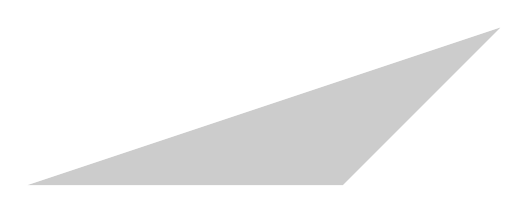
\begin{tikzpicture}
\fill[black!20!white](0,0)--(4,0)--(6,2)--(0,0);
\end{tikzpicture}}
\put(-60,-60){
\begin{tikzpicture}
\filldraw[left color=white,right color=black!20!white,draw=white]
(0,0)--(4.8,4.8)--(0.8,4.8)--(0,4.73)--(0,0);
\end{tikzpicture}}
% Axis system
\thinlines
\put(-60,0){\vector(1,0){120}}
\put(0,-60){\vector(0,1){120}}
\multiput(-50,-2)(25,0){5}{\line(0,1){4}}
\multiput(-2,-50)(0,25){5}{\line(1,0){4}}
\put(62,-1){$\alpha_m$}
\put(-1,61){$\alpha_f$}
\put(-55,-8){$-1$}
\put(-30,-8){$-\frac{1}{2}$}
\put(23.7,-8){$\frac{1}{2}$}
\put(48.7,-8){$1$}
\put(3,-51.5){$-1$}
\put(3,-26.5){$-\frac{1}{2}$}
\put(1, 27){$\frac{1}{2}$}
\put(3, 49){$1$}
\put(25,25){\line(-1,0){90}}
%
\thicklines
\put(25,25){\line(-1,-1){85}}
\put(25,25){\line(-3,-1){97}}
\put(0,0){\line(0,1){16.7}}
\put(-50,0){\line(1,0){50}}
\put(0,0){\circle*{1.5}}
\put(25,25){\circle*{1.5}}
\put(0,16.7){\circle*{1.5}}
\put(-50,0){\circle*{1.5}}
\put(-46,-50){$\lambda_{1,2}^\infty=-1$}
\put(-55,26.5){$\lambda_3^\infty=-1$}
\put(-82,-12){$\lambda_3^\infty=\lambda_{1,2}^\infty$}
%
\thinlines
\put(25,9){\vector(-1,0){24.5}}
\put(26,7){HHT-$\alpha$}
\put(-21,14){\vector(0,-1){4}}
\qbezier(25,40)(-21,30)(-21,14)
\put(26,39){Generalized-$\alpha$}
\end{picture}
\end{center}
\caption{Classification of the generalized-$\alpha$ method in the
$\alpha_m-\alpha_f$ space. From~\cite{HulbertChung}.}
\label{fig:GAstab}
\end{figure}

Inserting the internal force linearizations from \meqsref{eq:37}{eq:39} into
\eqnref{eq:GenAlphaEquil} and using $\Q_\kp1=\Q_k+\Delta\Q_k$,
we obtain the generalized-$\alpha$ equation on incremental form
%
\begin{equation}
\eqalign{
(1-\alpha_m){\mf M}_k\Delta\ddot{\mf r}_k + \Fi_k & \;+ \cr
(1-\alpha_f){\mf C}_k\Delta \dot{\mf r}_k + \Fd_k & \;+ \cr
(1-\alpha_f){\mf K}_k\Delta     {\mf r}_k + \Fs_k & \;=\;
(1-\alpha_f)\Delta\Q_k + \Q_k }
\end{equation}
%
or,
by collecting all known quantities of time increment $k$ on the right hand side
%
\begin{equation}
\eqalign{
(1-\alpha_m){\mf M}_k\Delta\ddot{\mf r}_k \;+\; &
(1-\alpha_f){\mf C}_k\Delta \dot{\mf r}_k \;+\;
(1-\alpha_f){\mf K}_k\Delta     {\mf r}_k \cr =\; &
(1-\alpha_f)\Delta\Q_k - \left(\Fi_k + \Fd_k + \Fs_k - \Q_k \right)
}\label{eq:IncGenAlphaEquil}
\end{equation}
%
The last term on the right hand side of \eqnref{eq:IncGenAlphaEquil} can be
recognized as the force residual of time increment $k$, and as such can be
omitted since this should be equal to zero if convergence has been achieved
before advancing to time increment $k+1$.

Inserting the Newmark incremental acceleration and velocity expressions from
\eqsref{eq:322}{eq:324} into \eqnref{eq:IncGenAlphaEquil} yields
%
\begin{equation}
\eqalign{
(1-\alpha_m){\mf M}_k&\left(
\frac{1}{\beta h^2} \Delta{\mf r}_k - {\mf a}_k - \ddot{\mf r}_k \right) \;+ \cr
(1-\alpha_f){\mf C}_k&\left(
\frac{\gamma}{\beta h} \Delta{\mf r}_k - {\mf d}_k - \dot{\mf r}_k \right) \;+ \cr
(1-\alpha_f){\mf K}_k&\Delta{\mf r}_k \;=\;
(1-\alpha_f)\Delta\Q_k - \left(\Fi_k + \Fd_k + \Fs_k - \Q_k \right) }
\end{equation}
%
which after rearranging the known quantities on the right hand side becomes
%
\begin{equation}
{\mf N}_k \Delta{\mf r}_k \;=\; \widehat{\mf R}_k
\end{equation}
%
with
%
\begin{equation}
{\mf N}_k \;=\;
\frac{1-\alpha_m}{\beta h^2}{\mf M}_k \;+\;
\frac{(1-\alpha_f)\gamma}{\beta h} {\mf C}_k \;+\;
(1-\alpha_f){\mf K}_k
\label{eq:NewtonGenAlpha}
\end{equation}
%
and
%
\begin{equation}
\eqalign{
\widehat{\mf R}_k \;=\; &
(1-\alpha_f)\Delta\Q_k - \left(\Fi_k + \Fd_k + \Fs_k - \Q_k \right) \cr +\; &
(1-\alpha_m){\mf M}_k({\mf a}_k + \ddot{\mf r}_k) \;+\;
(1-\alpha_f){\mf C}_k({\mf d}_k + \dot{\mf r}_k)
}\label{eq:PredictorGenAlpha}
\end{equation}

For a linear system, the state at time $t_\kp1$ given by $\Delta{\mf r}_k$,
$\Delta\dot{\mf r}_k$ and $\Delta\ddot{\mf r}_k$, and the associated inertia,
damping and elastic forces forces $\Fi_\kp1$, $\Fd_\kp1$ and $\Fs_\kp1$,
respectively, will satisfy the equilibrium \eqnref{eq:GenAlphaEquil}.
For nonlinear systems, the increments $\Delta{\mf r}_k$, $\Delta\dot{\mf r}_k$
and $\Delta\ddot{\mf r}_k$ will in general not satisfy
\eqnref{eq:GenAlphaEquil}.
In order to ensure dynamic equilibrium before advancing to the next time
increment, the dynamic residual seeks to be minimized through a similar
Newton--Raphson procedure as described in
Section~\ref{s:Newton-Raphson iteration}.
Thus, in each iteration we have to solve the linearized system of equations
%
\begin{equation}
\ls{i}{\mf N}_k \ls{i}\dr_k \;=\; \ls{i-1}{\mf R}^\alpha_k
\end{equation}
%
where the Newton matrix $\ls{i}{\mf N}_k$ is the same as in
\eqnref{eq:NewtonGenAlpha}, and the right-hand-side vector
$\ls{i-1}{\mf R}^\alpha_k$ equals
%
\begin{equation}
\eqalign{
\ls{i-1}{\mf R}^\alpha_k \;=\; &
(1-\alpha_f)\:\ls{i-1}\Q_\kp1  + \alpha_f\Q_k \cr -\; &
(1-\alpha_m)\,\ls{i-1}\Fi_\kp1 - \alpha_m\Fi_k \cr -\; &
(1-\alpha_f)\:\ls{i-1}\Fd_\kp1 - \alpha_f\Fd_k \cr -\; &
(1-\alpha_f)\:\ls{i-1}\Fs_\kp1 - \alpha_f\Fs_k
}\label{eq:CorrectorGenAlpha}
\end{equation}


%%%%%%%%%%%%%%%%%%%%%%%%%%%%%%%%%%%%%%%%%%%%%%%%%%%%%%%%%%%%%%%%%%%%%%%%%%%%%%%%
\section{Structural damping}
\label{s:Structural damping}
\label{sec:PropDamping}
\label{sec:RayleighDamping}

\iftoggle{publicedition}{% The following is for the public edition
The reduced superelement damping matrix
}{% The following is for the in-house edition only
The reduced superelement damping matrix, given by \eqnref{eqCMS:Csubs},
} % End in-house edition only
is not developed in Fedem.
Instead, proportional damping is used.
If we assume that the damping force in a superelement is proportional to the
velocity of each mass point, we have
%
\begin{equation}
{\mf c} \;=\; \alpha_1 {\mf m}
\end{equation}
%
where $\alpha_1$ is a constant.
Similarly, if we assume the damping force is proportional to the strain velocity
in each point, we have
%
\begin{equation}
{\mf c} \;=\; \alpha_2 {\mf k}
\end{equation}
%
where $\alpha_2$ is another constant.
The combination of these two assumptions produces the damping matrix of
{\it Rayleigh-damping} or {\it proportional damping}
%
\begin{equation}
{\mf c} \;=\; \alpha_1 {\mf m} + \alpha_2 {\mf k}
\label{eq:337}
\end{equation}

The damping ratio for the natural frequencies can now be calculated from
%
\begin{equation}
\lambda_i \;=\; \frac{1}{2}
\left( \frac{\alpha_1}{\omega_i} + \alpha_2 \omega_i \right)
\label{eq:338}
\end{equation}
%
where $\alpha_1$ damps out lower vibration modes
while $\alpha_2$ damps out higher modes.
If the damping ratios $\lambda_i$ for two vibration modes are selected,
the corresponding constants of proportionality, $\alpha_1$ and $\alpha_2$
may be calculated from
%
\begin{equation}
\eqalign{
\alpha_1 =\;& \frac{2 \omega_1 \omega_2}{\omega_2^2 - \omega_1^2}
\left( \lambda_1 \omega_2 - \lambda_2 \omega_1 \right) \cr
\alpha_2 =\;& \frac{2 \left( \omega_2 \lambda_2 - \omega_1 \lambda_1 \right)}
                   {\omega_2^2 - \omega_1^2}
}\label{eq:339}
\end{equation}
%
where $\omega_1$ and $\omega_2$ are the circle frequencies and $\lambda_1$ and
$\lambda_2$ are the damping ratios for the selected vibration modes,
see Figure~\ref{fig:RayleighDamping}.

\begin{figure}[b]
% SPDX-FileCopyrightText: 2023 SAP SE
%
% SPDX-License-Identifier: Apache-2.0
%
% This file is part of FEDEM - https://openfedem.org

%%%%%%%%%%%%%%%%%%%%%%%%%%%%%%%%%%%%%%%%%%%%%%%%%%%%%%%%%%%%%%%%%%%%%%%%%%%%%%%%
%
% FEDEM Theory Guide.
%
%%%%%%%%%%%%%%%%%%%%%%%%%%%%%%%%%%%%%%%%%%%%%%%%%%%%%%%%%%%%%%%%%%%%%%%%%%%%%%%%

\setlength{\unitlength}{1mm}
\begin{picture}(120,88)(-15,-10)
\thicklines
% Axis system
\put( 0, 0){\vector(1,0){95}}
\put( 0, 0){\vector(0,1){72}}
\multiput( 0, -1)(10, 0){10}{\line(0,1){2}}
\multiput( -1, 0)( 0,10){7}{\line(1,0){2}}
%
\put(-2,-5){$0.0$}
\put( 8,-5){$10$}
\put(18,-5){$20$}
\put(28,-5){$30$}
\put(38,-5){$40$}
\put(48,-5){$50$}
\put(58,-5){$60$}
\put(68,-5){$70$}
\put(78,-5){$80$}
\put(88,-5){$90$}
%
\put(-7,-1){$0.0$}
\put(-7, 9){$0.1$}
\put(-7,19){$0.2$}
\put(-7,29){$0.3$}
\put(-7,39){$0.40$}
\put(-7,49){$0.5$}
\put(-7,59){$0.6$}
%
\put(60,-10){\textsl{Circle frequency}}
\put(97,-1){$\omega$}
\put(-15,30){\rotatebox{90}{\textsl{Damping ratio}}}
\put(-1,74){$\lambda$}
\put(60, 8){\textsl{Asymptote: $\lambda = \frac{1}{2} \alpha_2 \omega$}}
\put( 5,55){\textsl{Asymptote: $\omega = 0$}}
\put(10,30){$\displaystyle\lambda = \frac{1}{2} \left( \frac{\alpha_1}{\omega}
             + \alpha_2 \omega \right)$}
%
%The actual damping function
\qbezier    ( 1.5,50.3)( 1.25,23.0)( 6.0,13.7)
\qbezier    ( 6.0,13.7)( 10.0,6.62)(20.0, 7.75)
\qbezier    (20.0, 7.75)(30.0, 8.4)(50.0,11.5)
\qbezier    (50.0,11.5)(75.0,15.7)(100.0,20.75)

\thinlines
\qbezier[200](  0.0,  0.0)( 50.0,  10.0)( 100.0, 20.0)
%
\qbezier[22](-10.0,  8.65)(  1.0,  8.65)( 12.0,  8.65)
\qbezier[60](-10.0, 11.5) ( 20.0, 11.5) ( 50.0, 11.5)
\qbezier[14]( 12.0, -5.0) ( 12.0,  1.8) ( 12.0,  8.65)
\qbezier[17]( 50.0, -5.0) ( 50.0,  3.2) ( 50.0, 11.5)
\put( 12.0, 8.65){\circle{2}}
\put( 50.0, 11.5){\circle{2}}
\put( 11.0,-10.0){$\omega_1$}
\put( 49.0,-10.0){$\omega_2$}
\put(-15.0, 7.65){$\lambda_1$}
\put(-15.0, 10.5){$\lambda_2$}
\end{picture}

\caption{A typical relationship between damping and natural frequency arising
from the specification of damping ratio at the frequencies.
($\alpha_1=1.5$ and $\alpha_2 = 0.004$).}
\label{fig:RayleighDamping}
\end{figure}

When using component modes (see Section~\ref{sec:CMS reduction}), the reduced
\iftoggle{publicedition}{% The following is for the public edition
superelement matrices are partitioned into sub-matrices associated with
the retained nodal DOFs and component modes, respectively.
}{% The following is for the in-house edition only
superelement mass- and stiffness matrices are partitioned
as given by \eqsref{eqCMS:Msubs}{eqCMS:Ksubs}, respectively.
} % End in-house edition only
It is then possible to assign individual Rayleigh damping factors for each
component mode.
In this case, exploiting that ${\mf k}_{12} = {\mf k}_{21}^T = {\mf 0}$
and ${\mf m}_{12} = {\mf m}_{21}^T$, \eqnref{eq:337} reads
%
\begin{equation}
\left[\begin{array}{cc}
{\mf c}_{11} & {\mf c}_{12} \\
{\mf c}_{21} & {\mf c}_{22}
\end{array}\right] \;=\;
\left[\begin{array}{cc}
\alpha_1 {\mf m}_{11} & \left( {\bm\alpha}_m {\mf m}_{21} \right)^T \\
{\bm\alpha}_m {\mf m}_{21} & {\bm\alpha}_m {\mf m}_{22}
\end{array}\right] +
\left[\begin{array}{cc}
\alpha_2 {\mf k}_{11} & {\mf 0} \\
{\mf 0} & {\bm\alpha}_k {\mf k}_{22}
\end{array}\right]
\end{equation}
%
where ${\bm\alpha}_m = \lceil\alpha_{mi}\rfloor$
and ${\bm\alpha}_k = \lceil\alpha_{ki}\rfloor$
are diagonal matrices containing the component mode damping factors.
Note that ${\mf m}_{22}$ and ${\mf k}_{22}$ both are diagonal matrices,
see Section~\ref{subsec:Reduced system}.

%%%%%%%%%%%%%%%%%%%%%%%%%%%%%%%%%%%%%%%%%%%%%%%%%%%%%%%%%%%%%%%%%%%%%%%%%%%%%%%%
\section{Evaluation of the Newton matrix}
\label{s:Evaluation of the Newton matrix}

The Newton matrix is a function of the integration parameters $\gamma$ and
$\beta$ and of the time increment size size $h$, see \eqnref{eq:327}.
In Section~\ref{sec:CMS reduction}, mass and stiffness matrices are developed
for each of the substructures and reduced to superelement matrices by
CMS-reduction techniques.
The tangent stiffness matrix of each substructure is then established at the
current configuration through the co-rotational formulation outlined in
Chapter~\ref{chap:SupElCorot}.

A superelement Newton matrix can now be calculated from the following relation
(refer to \eqsref{eq:327}{eq:337})
%
\begin{equation}
{\mf n}_i \;=\; {\mf k}_i
+ \frac{\gamma}{\beta h} \left( \alpha_1 {\mf m}_i + \alpha_2 {\mf k}_i \right)
+ \frac{1}{\beta h^2} {\mf m}_i
\label{eq:340}
\end{equation}
%
where
%
\begin{namelist}{xxx}
\item[${\mf n}_i$] reduced superelement Newton matrix
\item[${\mf k}_i$] reduced superelement stiffness matrix
\item[${\mf m}_i$] reduced superelement mass matrix
\end{namelist}

Each time the integration algorithm requires a new Newton matrix
(refer to \eqsref{eq:326}{eq:NewmarkDispCorr}),
the superelement Newton matrices are transformed to the actual directions
of the system level DOFs by
%
\begin{equation}
\bar{\mf n}_i \;=\; {\mf T}_{SEi}^T {\mf n}_i {\mf T}_{SEi}
\label{eq:341}
\end{equation}
%
resulting in the transformed superelement Newton matrix, $\bar{\mf n}_i$
\iftoggle{publicedition}{}{% The following is for the in-house edition only
(refer to
Sections~\ref{sec:SupElIntForce}--\ref{s:Substituting into system matrices})}.

The superelement Newton matrices are added into the incremental Newton matrix at
system level as indicated by
%
\begin{equation}
{\mf N}_k \;=\; \sum\limits_i {\mf a}_i^T \bar{\mf n}_i {\mf a}_i
\label{eq:342}
\end{equation}
%
where ${\mf a}_i$ are incidence matrices that represent superelement topology
\iftoggle{publicedition}{% The following is for the public edition
at system level.
}{% The following is for the in-house edition only
at system level (see also \eqsref{eqSC:512}{eqSC:513}).
} % End in-house edition only

The stiffness for a spring may be a constant or, in the nonlinear case,
a variable that is dependent on the spring deflection.
For axial springs, the stiffness is transformed to the directions of the
connected supernodes and then added directly to the Newton system matrix.
For joint springs, stiffness is added to the diagonal of the involved DOF
of the system's Newton matrix.

The damping coefficient of a damper may be a constant, or in the nonlinear case
a variable that is dependent on the damper velocity.
For the Newton matrix, the damping coefficient must be modified by the factor
$\frac{\gamma}{\beta h}$ (see \eqsref{eq:327}{eq:333}).
For axial dampers, the modified damping coefficient is transformed to the
actual directions for the connected supernodes and then added to the Newton
system matrix.
For joint dampers, the modified damping coefficients are added to the diagonal
of the involved DOF of the system's Newton matrix.

Additional masses may be regarded as constants during simulation.
For the Newton matrix, additional masses must be modified by the factor
$\frac{1}{\beta h^2}$ (refer to \eqsref{eq:327}{eq:333}).
The modified additional masses are added to the diagonal elements for the
specified DOFs of the Newton matrix.

%%%%%%%%%%%%%%%%%%%%%%%%%%%%%%%%%%%%%%%%%%%%%%%%%%%%%%%%%%%%%%%%%%%%%%%%%%%%%%%%
\section{Evaluation of the force vector}
\label{s:Evaluation of the force vector}

The force vector must be evaluated for each time increment and iteration (refer
to \eqsref{eq:326}{eq:NewmarkDispCorr}).
\iftoggle{publicedition}{}{% The following is for the in-house edition only
In addition to the contributions described in the sub-sections below,
the force vector may also contain buoyancy and hydrodynamic forces for beam
structures immersed in water.
These forces, and the associated tangent matrix contributions, are described in
Appendix~\ref{chap:Hydrodynamics}.
} % End in-house edition only

\subsection{External forces}
\label{subs:External forces}

The external forces at time increment $k+1$, $\Q_\kp1$
consist of the following contributions:
%
\begin{itemize}
\item Superelement gravitational forces
\item Concentrated external forces in supernodes
\item Gravitational forces from additional masses
\end{itemize}

The gravitational forces are transformed to actual directions of the DOFs at
\iftoggle{publicedition}{% The following is for the public edition
system level by means of the superelement transformation matrix ${\mf T}_{SEi}$
}{% The following is for the in-house edition only
system level by means of the transformation matrix~\eqref{eqSC:59}
} % End in-house edition only
%
\begin{equation}
\bar{\mf g}_i \;=\; {\mf T}_{SEi}^T {\mf g}_i
\label{eq:343}
\end{equation}
%
\iftoggle{publicedition}{}{% The following is for the in-house edition only
(see also \eqsref{eqSC:510}{eqSC:511}).
} % End in-house edition only
The transformed superelement's gravitational forces are then added
into the force vector by
%
\begin{equation}
\Q_\kp1 \;=\; \Q_\kp1 + \sum\limits_i {\mf a}_i^T \bar{\mf g}_i
\label{eq:344}
\end{equation}
%
\iftoggle{publicedition}{}{% The following is for the in-house edition only
(refer to \eqsref{eqSC:512}{eqSC:513}).
} % End in-house edition only

Direction and magnitude for specified concentrated loads are calculated for the
actual position of the mechanism, then transformed to the supernode direction
\iftoggle{publicedition}{}{% The following is for the in-house edition only
by the transformation matrix from \eqnref{eqSC:57} or~\eqref{eqSC:58},
} % End in-house edition only
and added into the system vector $\Q_\kp1$.
For loading on specified DOFs at system level, the magnitude at that position is
added directly into $\Q_\kp1$.

For additional masses added to translational DOFs, a gravitational force is
calculated by multiplying the component of the gravitational vector along the
actual DOF by the specified mass.
These gravitational forces are then added to $\Q_\kp1$ for the DOFs in question.

\subsection{Stiffness forces}

The superelement stiffness forces are
\iftoggle{publicedition}{}{% The following is for the in-house edition only
calculated as shown in Section~\ref{sec:SupElIntForce}. These forces are then}
transformed to the actual directions of the DOFs for superelement $i$, i.e.
%
\begin{equation}
\bar{\mf S}_i \;=\; {\mf T}_{SEi}^T {\mf S}_i
\label{eq:350}
\end{equation}
%
(see \eqnref{eq:343}) and formally added into the force vector by
%
\begin{equation}
\Fs \;=\; \sum\limits_i {\mf a}_i^T \bar{\mf S}_i
\label{eq:351}
\end{equation}
%
(see \eqnref{eq:344}).

In general, a spring element may have a stress-free length that is a function of
time, and it may also have a spring stiffness which is a function of the spring
deflection (see Section~\ref{s:Spring elements}).
At a given configuration of the mechanism, the specified stress-free length of
the spring, $l_0$, is evaluated and subtracted from the actual spring length,
$l$, to give the actual spring deflection
%
\begin{equation}
\delta \;=\; l({\mf r}) - l_0 (t)
\end{equation}

In a typical nonlinear case, the spring force is found by integrating the
stiffness over a change in the deflection.
For axial springs, the evaluated spring force is transformed to the direction of
the end supernodes and added into the force vector similar to
\eqsref{eq:350}{eq:351}.

For joint springs, the force (or torque) is calculated similarly to that of
axial springs; however, the force is added directly to the involved DOF of the
load vector without any further transformation.

\subsection{Inertia and damping forces}

Taking into account that
%
\begin{eqnarray}
\Fi_k &=& {\mf M}_k \ddot{\mf r}_k \label{eq:345} \\
\Fd_k &=& {\mf C}_k  \dot{\mf r}_k \label{eq:346}
\end{eqnarray}
%
the right-hand-side vector defined by \eqnref{eq:328} reduces to
%
\begin{equation}
\Delta\hat\Q_k \;=\;
\Q_\kp1 + {\mf C}_k{\mf d}_k + {\mf M}_k{\mf a}_k - \Fs_k
\label{eq:347}
\end{equation}
%
where ${\mf a}_k$ and ${\mf d}_k$ are the \textit{predicted} acceleration and
velocity, defined by \eqsref{eq:323}{eq:325}, respectively.

For the first iteration within each time increment, the effective inertia
forces are calculated by replacing $\ddot{\mf r}_k$ with $-{\mf a}_k$
in \eqnref{eq:345} and $\dot{\mf r}_k$ with $-{\mf d}_k$ in \eqnref{eq:346}.
To avoid assembling the system mass and damping matrix explicitly,
the corresponding superelement accelerations and velocities are extracted from
the system vectors and transformed to the local superelement direction.
The local superelement mass and damping matrices are then multiplied by the
corresponding local acceleration and velocity vectors to produce the
superelement inertia and damping forces, respectively.
These forces are then transformed to the actual supernode directions and added
into the system vector (compare with \eqsref{eq:343}{eq:344}).

In general, a damper element has a damping coefficient that is a function of the
damper velocity (see Section~\ref{s:Damper elements}).
For a given velocity, the damping coefficient and associated force or
torque is calculated.
The force/torque is then added directly to the involved DOF of the load vector
without any further transformation for joint dampers.
For axial dampers, the force is transformed in a similar manner as described
above for the axial springs.

The inertia forces (or torques) from additional masses on specified DOFs of the
mechanism are calculated by multiplying the DOF acceleration by the magnitude
of the mass.
These forces are then added to the corresponding DOFs of the load vector.

\subsection{Forces due to prescribed motion}

Prescribed motions in a mechanism can be imposed by introducing stiff springs
with a specified stress-free length variation as a function of time,
as described in Section~\ref{s:Spring elements}.
This is equivalent to a penalty-enforcement of the motion constraint,
where the spring stiffness serves as the penalty parameter.

In Fedem, it is also possible of enforce the prescribed motion explicitly,
by eliminating the DOF that is prescribed from the system of
\eqsref{eq:326}{eq:NewmarkDispCorr}.
This is usually more efficient, since the number of unknowns then is reduced,
and it may also yield a more stable solution process since we don't have to
deal with penalty parameters.
It is possible to prescribe motions in joint DOFs or directly on triads.

For a given DOF $n$, we assume that the motion in terms of total displacement
relative to the initial position is a known function of time, $u_n = u_n(t)$.
%
The right-hand-side vector of the equation system~\eqref{eq:326}, given by
\eqnref{eq:347} above, is then modified as follows
%
\begin{equation}
\eqalign{
\Delta\hat\Q_k =\; &
\Q_\kp1 - {\mf N}_k {\bm\delta}_n \Delta u_k +
{\mf C}_k{\mf d}_k + {\mf M}_k{\mf a}_k - \Fs_k
}\label{eq:352}
\end{equation}
%
where $\Delta u_k = u_n(t_\kp1) - u_n(t_k)$ is the increment in the prescribed
motion from the previous time increment, $k$, to the next increment, $k+1$,
and ${\bm\delta}_n$ is a constant vector with the value 1 at the location
corresponding to the prescribed DOF $n$, and zero elsewhere.
The size of the equation system~\eqref{eq:326} is then reduced by 1, by removing
the $n$'th column and row of the Newton matrix and the right-hand-side vector,
since this DOF no longer is an unknown.

The equation system of the iterations~\eqref{eq:NewmarkDispCorr} is modified in
a similar manner, except that there is no additional force term here since the
iterative correction on the prescribed DOF, $\ls{i}\Delta u_k$, by definition
always is zero.

One can also use a prescribed velocity or acceleration in the same manner.
We then use the Newmark integration parameters to derive the equivalent
prescribed displacement, which then is inserted into \eqnref{eq:352}.
With a prescribed velocity function $v_n(t)$,
we find the equivalent displacement increment to impose from \eqnref{eq:324} as
%
\begin{equation}
\Delta u_k \;=\; \frac{\beta h}{\gamma}\left(v_n(t_\kp1) - v_n(t_k)\right) +
h\,v_n(t_k) + \left(\frac{1}{2}-\frac{\beta}{\gamma}\right)h^2 \ddot{r}_k
\end{equation}
%
Similarly, with a prescribed acceleration function $a_n(t)$,
we can find an equivalent displacement from \eqnref{eq:322} as
%
\begin{equation}
\Delta u_k \;=\; \beta h^2 \left(a_n(t_\kp1) - a_n(t_k)\right) +
h\,\dot{r}_k + \frac{h^2}{2}a_n(t_k)
\end{equation}


\clearpage
%%%%%%%%%%%%%%%%%%%%%%%%%%%%%%%%%%%%%%%%%%%%%%%%%%%%%%%%%%%%%%%%%%%%%%%%%%%%%%%%
\section{Quasi-static equilibrium}
\label{s:Quasi-static equilibrium}

Dynamic simulation of mechanism motion should start from an equilibrium position
to avoid that unbalanced forces in the mechanism from the initial configuration
cause a false superimposed vibration in the simulation results.
This can happen when the simulation starts from both a stationary position and
a position with initial velocities and acceleration.
Unbalanced forces for the stationary position arise from gravitation forces,
initially loaded springs and initial external loading, as well as from
positioning inaccuracies in the mechanism modeling.
Equilibrium for the initial positions of mechanisms with initial velocities and
accelerations also includes the unbalanced inertia and damping forces.

The inclusion of possible inertia and damping effects in the initial equilibrium
iteration justifies the term {\it quasi-static equilibrium} iteration.
Since the initial velocities and accelerations are either zero or specified,
their correction in the inertia and damping terms on the left-hand side of the
iteration \eqnref{eq:NewtonDynEq} cancel out.
The quasi-static iteration equation therefore reduces to
%
\begin{equation}
\ls{i}{\mf K}_0 \ls{i}\dr_0 \;=\; \ls{i-1}\Q_0 - \left[
\ls{i-1}\Fi_0 + \ls{i-1}\Fd_0 + \ls{i-1}\Fs_0 \right]
\label{eq:QSE}
\end{equation}
%
Here, the subindices have been changed to $0$, indicating the initial position.
In the case of prescribed motion, the first iteration is instead governed by
%
\begin{equation}
{}^1{\mf K}_0 {}^1\dr_0 \;=\; {}^0\Q_0 - \left[
{}^1{\mf K}_0 {\bm\delta}_n u_n(t_0) + {}^0\Fi_0 + {}^0\Fd_0 + {}^0\Fs_0 \right]
\end{equation}

If the rigid body mechanism motions all are either constrained by springs---as
in a car suspension system---or fixed, the stiffness matrix is nonsingular and
\eqnref{eq:QSE} may be used to iterate for the equilibrium position.
When mechanism motion is controlled by force input, \eqnref{eq:QSE} may
be singular and {\it additional boundary conditions} must be introduced
into the equation to eliminate the rigid body DOFs of the mechanism.
In this case, extra boundary conditions that are effective for the quasi-static
equilibrium iterations only, are usually specified for DOFs where the external
forces are applied.
This modifies \eqnref{eq:QSE} so that it becomes nonsingular, and the
iteration can proceed until equilibrium is reached within a specified tolerance.

\clearpage
\subsection{Equilibrium iteration procedure}

Starting from \eqnref{eq:QSE}, possibly modified by additional boundary
conditions, the iteration will follow the same algorithm as in the dynamic
equilibrium iteration described above, with the exception that the stiffness
matrix ${\mf K}_0$ replaces the Newton matrix from the dynamic case.
For each iteration the initial position of the mechanism is improved from
%
\begin{equation}
\ls{i}{\mf r}_0 \;=\; \ls{i-1}{\mf r}_0 + \ls{i}\dr_0
\end{equation}
%
The updating of the velocity and acceleration vector in the dynamic iteration
procedure is omitted in the quasi-static case.
The stiffness matrix is evaluated in the same way as the Newton matrix described
in Section~\ref{s:Evaluation of the Newton matrix}.
All the stiffness terms from superelement matrices and springs are kept,
while the mass and damping terms from superelement matrices, additional masses,
and dampers are skipped.

The external force vector $\ls{i-1}\Q_0$ in \eqnref{eq:QSE}
is evaluated in the same way as in the dynamic case for the initial time.
The inertia and damping forces, $\ls{i-1}\Fi_0$ and $\ls{i-1}\Fd_0$,
are evaluated based on constant velocities and accelerations during iteration.
However, these vectors may also change during iteration due to updated positions
of the mechanism.
The stiffness forces $\ls{i-1}\Fs_0$ are evaluated in exactly the same way
as in the dynamic case.

The iteration based on \eqnref{eq:QSE} is called Newton--Raphson
iteration, or modified Newton--Raphson if the stiffness matrix is kept constant
during some or all iterations.
If the stiffness matrix is kept constant during iteration, the last evaluated
and triangularized stiffness matrix is kept for new iterations.
Only the right-hand-side vector of \eqnref{eq:QSE} is then evaluated
for each iteration, and the increments for improving the mechanism position
are evaluated through backward substitution.
When many iterations are necessary, this can save computational effort.

% SPDX-FileCopyrightText: 2023 SAP SE
%
% SPDX-License-Identifier: Apache-2.0
%
% This file is part of FEDEM - https://openfedem.org

%%%%%%%%%%%%%%%%%%%%%%%%%%%%%%%%%%%%%%%%%%%%%%%%%%%%%%%%%%%%%%%%%%%%%%%%%%%%%%%%
%
% FEDEM Theory Guide.
%
%%%%%%%%%%%%%%%%%%%%%%%%%%%%%%%%%%%%%%%%%%%%%%%%%%%%%%%%%%%%%%%%%%%%%%%%%%%%%%%%

\def\eiot{e^{i\omega t}}
\clearpage

%%%%%%%%%%%%%%%%%%%%%%%%%%%%%%%%%%%%%%%%%%%%%%%%%%%%%%%%%%%%%%%%%%%%%%%%%%%%%%%%
\section{Frequency Response Analysis}
\label{s:Frequency Response Analysis}

Frequency response analysis is an alternative approach to compute the structural
response due to steady state excitation given in the frequency domain.
The excitations are applied forces and/or motions,
like displacements, velocities or accelerations.
Two types of analysis are available~\cite{Brincker}:
%
\begin{itemize}
%
\item{\it Direct frequency response} \mdash The response will be computed
by solving a set of coupled equations by using complex arithmetics.
%
\item{\it Modal frequency response} \mdash This method uses the decomposition
based on eigenmodes. A certain number of modes, called the eigenspace,
will be used for the response calculation and reduces the overall system size.
%
\end{itemize}
%
In the end, the modal frequency response will yield exactly the same answer as
the direct frequency response, provided that all modal degrees of freedom are
included in the analysis. However, the strength of the modal approach comes from
the idea that the solution is very close to the direct approach by using
significantly fewer modal degrees of freedom than physical degrees of freedom.

%%%%%%%%%%%%%%%%%%%%%%%%%%%%%%%%%%%%%%%%%%%%%%%%%%%%%%%%%%%%%%%%%%%%%%%%%%%%%%%%
\subsection{Direct frequency response analysis}
\label{subs:Direct frequency response analysis}

In direct frequency response analysis, the response is computed at discrete
excitation frequencies by solving a set of coupled matrix equations.
The equation of damped forced vibration with harmonic excitation is given by:
%
\begin{equation}
\label{eq:fra0}
{\mf M}\ddot{\mf r}(t) + {\mf C}\dot{\mf r}(t) + {\mf K}{\mf r}(t) \;=\;
{\mf P}(\omega)\eiot
\end{equation}
%
The load in \eqnref{eq:fra0} is introduced as a complex vector,
which is more convenient to solve for. From the physical point of view,
the load can be real or imaginary, or both.

For harmonic motion (which is the basis of a frequency response analysis),
a harmonic solution of the following form will be assumed:
%
\begin{equation}
\label{eq:fra1}
{\mf r}(t) \;=\; {\mf u}(\omega)\eiot
\end{equation}
%
where ${\mf r}(t)$ is the complex displacement vector,
and $\omega$ is the circle frequency of the periodic load and response.
Taking the first and second derivatives of \eqnref{eq:fra1},
the following is obtained:
%
\begin{eqnarray}
\label{eq:fra2}
\dot{\mf r}(t) &=& \;\:i\omega\:{\mf u}(\omega)\eiot \\
\label{eq:fra3}
\ddot{\mf r}(t) &=& \!-\omega^2{\mf u}(\omega)\eiot
\end{eqnarray}
%
When the above expressions are substituted into \eqnref{eq:fra0}, we obtain:
%
\begin{equation}
\label{eq:fra4}
-\omega^2{\mf M u}(\omega)\eiot +
i\omega  {\mf C u}(\omega)\eiot +
         {\mf K u}(\omega)\eiot \;=\; {\mf P}(\omega)\eiot
\end{equation}
%
which simplifies to
%
\begin{equation}
\label{eq:fra5}
-\omega^2{\mf M}{\mf u}(\omega) +
 i\omega {\mf C}{\mf u}(\omega) +
         {\mf K}{\mf u}(\omega) \;=\; {\mf P}(\omega)
\end{equation}

The expression~\eqref{eq:fra5} represents a system of equations with complex
coefficients if damping is included or the applied loads have phase angles.
This equation of motion is solved for given forcing frequencies, $\omega$,
in the same manner as for linear static problems, but using complex arithmetics.

%%%%%%%%%%%%%%%%%%%%%%%%%%%%%%%%%%%%%%%%%%%%%%%%%%%%%%%%%%%%%%%%%%%%%%%%%%%%%%%%
\subsection{Modal frequency response analysis}
\label{subs:Modal frequency response analysis}

The modal frequency response analysis method
uses the mode shapes of the structure to reduce the size of the equation system.
It uncouples the equations of motion thereby making the numerical solution more
efficient. Since the mode shapes typically are computed as part of the
characterization of the structure, modal frequency response is a natural
extension of a normal mode analysis.

As a first step in the formulation, the variables are transformed from physical
coordinates ${\mf u}(\omega)$ to modal coordinates by assuming
%
\begin{equation}
\label{eq:fra6}
{\mf u}(\omega) \;=\; {\pmb\phi}\,{\pmb\xi}(\omega)\eiot
\end{equation}
%
The \eqnref{eq:fra6} represents an equality if all modes are used.
However, since that rarely is the case the equation represents an approximation.
Substituting the modal coordinates in \eqnref{eq:fra6} for the physical
coordinates in \eqnref{eq:fra5} and simplifying, the following is obtained:
%
\begin{equation}
\label{eq:fra8}
-\omega^2{\mf M}{\pmb\phi}\,{\pmb\xi}(\omega) +
i\omega  {\mf C}{\pmb\phi}\,{\pmb\xi}(\omega) +
         {\mf K}{\pmb\phi}\,{\pmb\xi}(\omega) \;=\; {\mf P}(\omega)
\end{equation}
%
which represents the equation of motion in modal coordinates.

At this point the equations remain coupled.
To uncouple the equations, premultiply by ${\pmb\phi}^T$ to obtain
%
\begin{equation}
\label{eq:fra9}
-\omega^2{\pmb\phi}^T{\mf M}{\pmb\phi}\,{\pmb\xi}(\omega) +
  i\omega{\pmb\phi}^T{\mf C}{\pmb\phi}\,{\pmb\xi}(\omega) +
         {\pmb\phi}^T{\mf K}{\pmb\phi}\,{\pmb\xi}(\omega) \;=\;
         {\pmb\phi}^T{\mf P}(\omega)
\end{equation}
%
where the expressions represent:
%
\begin{eqnarray*}
{\pmb\phi}^T{\mf M}\,{\pmb\phi}\!\! &:& \mbox{modal mass matrix\hskip3cm} \\
{\pmb\phi}^T{\mf C}\,{\pmb\phi} &:& \mbox{modal damping matrix} \\
{\pmb\phi}^T{\mf K}\,{\pmb\phi} &:& \mbox{modal stiffness matrix} \\
{\pmb\phi}^T{\mf P}\;\;\;       &:& \mbox{modal load vector}
\end{eqnarray*}

The final step uses the orthogonality property of the mode shapes to
formulate the equation of motion in terms of the generalized mass, damping and
stiffness matrices, which are diagonal matrices (damping as long as it is
defined as a linear combination between the stiffness and mass matrix).
Therefore, in this form the modal equations of motion are uncoupled.
In this uncoupled form, the equations of motion are written as a set of
scalar equations, like
%
\begin{equation}
\label{eq:fra10}
-\omega^2\,m_i\,{\xi_i}(\omega) +
i\omega  \,c_i\,{\xi_i}(\omega) +
           k_i\,{\xi_i}(\omega) \;=\; p_i(\omega)
\end{equation}
%
where
%
\begin{eqnarray*}
m_i\! &:& i^{th}\mbox{ modal mass\hskip6cm} \\
c_i &:& i^{th}\mbox{ modal damping} \\
k_i &:& i^{th}\mbox{ modal stiffness} \\
p_i &:& i^{th}\mbox{ modal load}
\end{eqnarray*}

The modal form is much faster to solve than the direct method
because it is a series of uncoupled single-degree-of-freedom equations.
Once the individual modal responses are computed, physical responses are
recovered as the summation of the modal responses using \eqnref{eq:fra6}.
These responses are in complex form (magnitude/phase or real/imaginary).

%%%%%%%%%%%%%%%%%%%%%%%%%%%%%%%%%%%%%%%%%%%%%%%%%%%%%%%%%%%%%%%%%%%%%%%%%%%%%%%%
\subsection{Modal vs. direct frequency response}
\label{subs:Modal vs. direct frequency response}

Some general guidelines can be used when selecting modal frequency
response analysis versus direct frequency response analysis.
These guidelines are summarized in table~\ref{tab:ModalDirectFreq}.

\begin{table}[b]
  \caption{Modal vs. Direct Frequency Response}
  \label{tab:ModalDirectFreq}
  \begin{center}
    \begin{tabular}{lcc}
      \hline
      & Modal & Response \\
      \hline
      Small model & & x \\
      Large model & x & \\
      Few excitation frequencies & & x \\
      Many excitation frequencies & x & \\
      High frequency excitation & & x \\
      Nonmodal damping & & x \\
      Higher accuracy & & x \\
      \hline
    \end{tabular}
  \end{center}
\end{table}

In general, larger models may be solved more efficiently in modal frequency
response because the numerical solution is a solution of a smaller system of
uncoupled equations.
The modal method is particularly advantageous if the natural frequencies and
mode shapes were computed during a previous stage of the analysis.
In that case, you simply perform a recover/restart.
Using the modal approach to solve the uncoupled equations is very efficient,
even for very large numbers of excitation frequencies.

On the other hand, the major portion of the effort in a modal frequency response
analysis is the calculation of the modes.
For large systems with a large number of modes, this operation can be as
costly as a direct solution.
This result is especially true for high-frequency excitation.
To capture high frequency response in a modal solution, less accurate,
high-frequency modes must be computed.
For small models with a few excitation frequencies, the direct method may be the
most efficient because it solves the equations without first computing modes.
The direct method is also more accurate than the modal method because the direct
method is not concerned with mode truncation.

%%%%%%%%%%%%%%%%%%%%%%%%%%%%%%%%%%%%%%%%%%%%%%%%%%%%%%%%%%%%%%%%%%%%%%%%%%%%%%%%
\subsection{Sampling and windowing}
\label{subs:Sampling and windowing}

The sampling rate defines the upper limit on the frequency that can be
used for analysis of the input data, i.e., the forcing function.
It describes the number of data samples acquired per unit time.
The sampling rate is also denoted as sampling frequency.
%E.g. is the input aquired at a sampling frequency of 100 Hz,
The upper limit of the frequency band is given by the Nyquist frequency, $f_q$
%
\begin{equation}
f_q = \frac{f_s}{2} \quad\mbox{and}\quad f_s = \frac{1}{\Delta t_s}
\end{equation}
%
where $f_s$ is the sampling frequency
and $\Delta t_s$ is the sampling time increment.
E.g., if the sampling frequency is 100~Hz, then the investigations are limited
to 50~Hz and any information beyond this frequency can not be determined.
This means that the sampling frequency must be chosen large enough
to get the desired information from the input data.

Handling large amounts of input data can be done via {\it segmenting},
which reduces the leakage in subsequent fourier transformations
while minimizing discontinuities between the data segments.
The duration of each segment is defined by
%
\begin{equation}
\label{eq:wtime}
T_w \;=\; N_w\,\Delta t
\end{equation}
%
where $N_w$ denotes the number of samples in each window.
The segmenting procedure consists of multiplying the input data by a
finite-length windowing function with an amplitude that varies smoothly and
gradually toward zero at the edges.
In Fedem, the Hanning window (raised-cosine window) is used.
This windowing function, which is depicted in Figure~\ref{fig:Hanning}, can be
seen as one period of a cosine `raised' so that negative peaks just touch zero.
%
\begin{figure}[b]
\includegraphics[width=\textwidth]{Figures/hanning300}
\caption{The Hanning window.}
\label{fig:Hanning}
\end{figure}

Figure~\ref{fig:Sample Input} shows a sample input data sequence,
for simplicity just a sine function.
%
\begin{figure}[tb]
\includegraphics[width=\textwidth]{Figures/input}
\caption{Sample input data.}
\label{fig:Sample Input}
\end{figure}
%
Each data segment will then be captured by overlapping and window tapering
such that the sum of all data segments is equal to the original,
except at the ends where the window is still present.
An easy way to accomplish this is to use the Hanning window with 50\% overlap,
as showed in Figure~\ref{fig:Overlapping Hanning}.
%
\begin{figure}[!tb]
\center
\includegraphics[width=\textwidth]{Figures/movingHenning}
\caption{Three Hanning windows with 50\% overlap.}
\label{fig:Overlapping Hanning}
\end{figure}
%
The additional dashed black line represents the superposition of the overlapped
windows, which results in unity except for at the ends of the sequences where
the window is still present.
Figure~\ref{fig:Tapered data} shows the tapered data segments for three
Hanning windows, which are obtained by multiplying the window function
with the input data-sequence.
The product is zero-valued outside the interval.
All that is left is the part where they coincide,
the ``view through the window''.
This input data isolation (tapering) is the main purpose of window functions.
%
\begin{figure}[tb]
\includegraphics[width=\textwidth]{Figures/tapered}
\caption{Tapered windows.}
\label{fig:Tapered data}
\end{figure}

It is convenient to perform the windowing and overlapping between segments in
such a way that the windowed data segments are defined in terms of the
absolute time, i.e.,
%
\begin{equation}
\label{eq:wind}
y_k(t) \;=\:
\begin{cases}
y(t)\,\omega(t-t_k) & t\subset\left[t_k,t_k+T\right] \\
      0             & t\not\subset\left[t_k,t_k+T\right]
\end{cases}
\end{equation}
%
For each of these tapered windows, a Fast Fourier Transform (FFT) into the
frequency domain, and an inverse FFT back to time domain will be applied.
After assembling, the `tapered system response'
(see Figure~\ref{fig:Tapered system response}) will be obtained.
As mentioned above, at the ends the window lobes are still active.
%
\begin{figure}[tb]
\includegraphics[width=\textwidth]{Figures/response}
\caption{Tapered system response}
\label{fig:Tapered system response}
\end{figure}
%
The systems response in Figure~\ref{fig:Tapered system response}
is based on an undamped system.
The transfer function reduces the amplitude, and there is no phase shift
because the system is undamped and not in resonance.

The window size $N_w$ represents the number of samples and herefrom the
duration $T_w$ (see \eqnref{eq:wtime}).
It depends on the fundamental frequency, intensity and change. In general:
{\it The lower the frequency, the bigger the window size should be.}
The default behaviour in Fedem is to not use windowing and to treat the entire
time series of the simulation in one go.

%%%%%%%%%%%%%%%%%%%%%%%%%%%%%%%%%%%%%%%%%%%%%%%%%%%%%%%%%%%%%%%%%%%%%%%%%%%%%%%%
\subsection{Fast fourier transformation (FFT)}
\label{subs:Fast fourier transformation}

A Fourier transform takes a signal in the time domain and
switches it into the frequency domain, e.g., it transforms a time series
$f(t)$ of $N$ equally- or uniformly spaced points in time $t_n=n\Delta t$,
$n=0,\ldots,N-1$, from the discrete time (or spatial) domain
to the discrete frequency domain.
The inverse Fourier transform does the inverse transformation from the
frequency domain back to the time (or spatial) domain.

The discrete Fourier transform (DFT) is defined given by
%
\begin{equation}
\label{eq:dft_sum0}
X_k \;=\; \sum_{n=0}^{N-1} x_n e^{-{i2\pi kn}/N}
\end{equation}
%
where $x_n$ are the values of a signal at equally spaced times $n=0,\ldots,N-1$.
The output $X_k$ is a complex number which encodes the amplitude and phase of a
sinusoidal wave with frequency $k/N$ cycles per time unit\footnote{This comes
from Euler's formula:
$\exp(\frac{i2\pi kn}{N}) = \cos(\frac{2\pi kn}{N}) + i\sin(\frac{2\pi kn}{N})
$.}.
The effect of computing $X_k$ is to find the coefficients of a signal
approximation by a linear combination of such waves.
Since each wave has a whole number of cycles per $N$ time units,
the approximation will be periodic with period $N$.
This approximation is given by the inverse Fourier transform
%
\begin{equation}
\label{eq:dft_sum1}
x_n \;=\; \frac{1}{N} \sum_{k=0}^{N-1} X_k e^{i2\pi kn}/N
\end{equation}
%
with
%
\vskip\baselineskip
\begin{namelist}{$n/N$}
\item[$N$] number of time samples
\item[$n$] current sample ($0,\ldots,N-1$)
\item[$x_n$] value of the signal at time $t_n$
\item[$k$] current frequency from 0 Hz up to $N-1$ Hz
\item[$X_k$] amount of frequency $k$ in the signal (amplitude and phase)
\item[$1/N$] normalization factor
\item[$n/N$] percent of "going through" time, $2\pi k$ speed in radians/sec
\end{namelist}
%
\vskip0.5\baselineskip
The DFT can be efficiently computed by the Fast Fourier Transform (FFT) algorithm.

\subsubsection{Units and spacing}

Let $\Delta t$ denote the spacing between points in time
and $N$ be the number of points/time samples.
The spacing $\Delta f$ of the points in frequency is the $1/(N\Delta t)$.
The quantity $1/\Delta t$ is called the sampling frequency $f_s$,
which should be at least twice of the highest frequency that is present in the
underlying continuous signal.

\subsubsection{Nyquist frequency, aliasing, mirroring}

When all frequencies present in the underlying continuous signal are below the
Nyquist frequency $f_q=\frac{1}{2\Delta t}$, then the discretely sampled time
series contains all of the information in the original continuous signal.
This is known as the sampling theorem and is a remarkable fact.

If a frequency exceeds the Nyquist frequency, the power from that frequency is
still transferred to the FFT, but it gets mapped to a bin in the result as if it
had been wrapped around. This phenomena is termed aliasing.
One can think of the resulting spectrum as being a circular buffer, representing
signal at each frequency modulo the maximum frequency of $\frac{1}{\Delta t}$.
A frequency of $\frac{1}{2\Delta t}$ would map to the middle bin,
also frequencies of $\frac{3}{2\Delta t}$, $\frac{5}{2\Delta t}$ and so on.

\subsubsection{Amplitude and phase}

Each number in the result of FFT is a complex number, an encoding of both the
amplitude and phase shift of each frequency component.
For example, if a 200 Hz component is present, the magnitude of the result at
200 Hz (as given by the absolute value of complex numbers) gives the power
density at that frequency.
For recovering the original signal, the phase of the component is also relevant.
Even though the power density at a certain frequency $f$ is the same for a
$\sin(2\pi ft)$, a $\cos(2\pi ft)$, or a $\sin(2\pi ft + \phi_0)$,
the phase is different in each of these cases.

The absolute height of an FFT is sometimes confusing.
The FFT reflects the total energy of the signal,
including the positive and negative frequencies.
Only the positive frequencies are from interest and therefore for
getting the amplitudes of the input, the FFT must be multiplied by 2.

\subsubsection{Efficiency}

The FFT algorithm is a fast implementation of the Discrete Fourier Transform
(DFT), which is most efficient when the number of elements $N$ in $t$ and $f$
is an even power of 2.
The worst efficiency will occur if $N$ is a prime number,
the efficiency of the FFT decreases to the efficiency of the DFT itself.
A DFT requires $O(N^2)$ steps, a FFT requires $O(N\log(N))$ steps.

%%%%%%%%%%%%%%%%%%%%%%%%%%%%%%%%%%%%%%%%%%%%%%%%%%%%%%%%%%%%%%%%%%%%%%%%%%%%%%%%
\subsection{Modal damping}
\label{subs:Modal Damping}

Finding proper specification for the structural damping is one of the most
challenging input tasks, because verification is possible only by performing
a response analysis in the time domine.
One way to specify the damping is by means of modal damping,
where the frequency-dependent damping ratio as the percentage of the critical
damping is specified for each mode.
This will then result in a diagonal damping matrix associated with the modes.

The modal damping ratio can be calculated via
%
\begin{equation}
\label{eq:modal_damping}
\zeta_i \;=\; \frac{c_i}{c_{{\rm cr},i}}
\end{equation}
%
with the critical damping $c_{{\rm cr},i}=2m_i\omega_i$
and $\omega_i^2=\frac{k_i}{m_i}$.
The important characteristic in modal damping reflects that the damping values
are calculated at natural frequencies and not at the excitation frequencies.

